% abtex2-modelo-artigo.tex, v-1.9.2 laurocesar
% Copyright 2012-2014 by abnTeX2 group at http://abntex2.googlecode.com/ 
%

% ------------------------------------------------------------------------
% ------------------------------------------------------------------------
% abnTeX2: Modelo de Artigo Acadêmico em conformidade com
% ABNT NBR 6022:2003: Informação e documentação - Artigo em publicação 
% periódica científica impressa - Apresentação
% ------------------------------------------------------------------------
% ------------------------------------------------------------------------


% ------------------------------------------------------------------------
% Modelo de pré-projeto para TCC 
% Universidade Federal do Piauí - CSHNB
% ------------------------------------------------------------------------



\documentclass[
	% -- opções da classe memoir --
	article,			% indica que é um artigo acadêmico
	11pt,				% tamanho da fonte
	oneside,			% para impressão apenas no verso. Oposto a twoside
	a4paper,			% tamanho do papel. 
	% -- opções da classe abntex2 --
	%chapter=TITLE,		% títulos de capítulos convertidos em letras maiúsculas
	%section=TITLE,		% títulos de seções convertidos em letras maiúsculas
	%subsection=TITLE,	% títulos de subseções convertidos em letras maiúsculas
	%subsubsection=TITLE % títulos de subsubseções convertidos em letras maiúsculas
	% -- opções do pacote babel --
	english,			% idioma adicional para hifenização
	brazil,				% o último idioma é o principal do documento
	sumario=tradicional
	]{abntex2}


% ---
% PACOTES
% ---

% ---
% Pacotes fundamentais 
% ---
\usepackage{lmodern}			% Usa a fonte Latin Modern
\usepackage[T1]{fontenc}		% Selecao de codigos de fonte.
\usepackage[utf8]{inputenc}		% Codificacao do documento (conversão automática dos acentos)
\usepackage{indentfirst}		% Indenta o primeiro parágrafo de cada seção.
\usepackage{nomencl} 			% Lista de simbolos
\usepackage{color}				% Controle das cores
\usepackage{graphicx}			% Inclusão de gráficos
\usepackage{microtype} 			% para melhorias de justificação
% ---
		
% ---
% Pacotes adicionais, usados apenas no âmbito do Modelo Canônico do abnteX2
% ---
\usepackage{lipsum}				% para geração de dummy text
% ---
		
% ---
% Pacotes de citações
% ---
\usepackage[brazilian,hyperpageref]{backref}	 % Paginas com as citações na bibl
\usepackage[alf]{abntex2cite}	% Citações padrão ABNT
% ---

% ---
% Configurações do pacote backref
% Usado sem a opção hyperpageref de backref
\renewcommand{\backrefpagesname}{Citado na(s) página(s):~}
% Texto padrão antes do número das páginas
\renewcommand{\backref}{}
% Define os textos da citação
\renewcommand*{\backrefalt}[4]{
	\ifcase #1 %
		Nenhuma citação no texto.%
	\or
		Citado na página #2.%
	\else
		Citado #1 vezes nas páginas #2.%
	\fi}%
% ---

% ---
% Informações de dados para CAPA e FOLHA DE ROSTO
% ---
\titulo{Título do Trabalho de Conclusão de Curso}
\autor{
	Aluno: Esdras Fragoso da Silva Neto (CPF:057.886.133-02)
	\\
	E-mail:esdrasfragoso@gamil.com; Período da Graduação: VII
	\\
	Orientador: Frank Cesar Lopes Veras
}
% ---

% ---
% Configurações de aparência do PDF final

% alterando o aspecto da cor azul
\definecolor{blue}{RGB}{41,5,195}

% informações do PDF
\makeatletter
\hypersetup{
     	%pagebackref=true,
		pdftitle={\@title}, 
		pdfauthor={\@author},
    	pdfsubject={Modelo de artigo científico com abnTeX2},
	    pdfcreator={LaTeX with abnTeX2},
		pdfkeywords={abnt}{latex}{abntex}{abntex2}{atigo científico}, 
		colorlinks=true,       		% false: boxed links; true: colored links
    	linkcolor=blue,          	% color of internal links
    	citecolor=blue,        		% color of links to bibliography
    	filecolor=magenta,      		% color of file links
		urlcolor=blue,
		bookmarksdepth=4
}
\makeatother
% --- 

% ---
% compila o indice
% ---
\makeindex
% ---

% ---
% Altera as margens padrões
% ---
\setlrmarginsandblock{3cm}{3cm}{*}
\setulmarginsandblock{3cm}{3cm}{*}
\checkandfixthelayout
% ---

% --- 
% Espaçamentos entre linhas e parágrafos 
% --- 

% O tamanho do parágrafo é dado por:
\setlength{\parindent}{1.3cm}

% Controle do espaçamento entre um parágrafo e outro:
\setlength{\parskip}{0.2cm}  % tente também \onelineskip

% Espaçamento simples
\SingleSpacing

% ----
% Início do documento
% ----
\begin{document}

% Retira espaço extra obsoleto entre as frases.
\frenchspacing 

% ----------------------------------------------------------
% ELEMENTOS PRÉ-TEXTUAIS
% ----------------------------------------------------------


% página de titulo
\maketitle


% resumo em português
\begin{resumoumacoluna}
	
 \textbf{Contexto:} A presença da informática na educação, em especial no ensino básico, vem sendo intensificada nos países desenvolvidos, que passaram a utilizar uma gama de instrumentos tecnológicos para melhoria do ensino e aprendizado. No Brasil, a utilização de Tecnologia da Informação – TI na educação tem ganhado mais espaço gradativamente. \\
 \textbf{Problema:} No entanto, diferente dos países desenvolvidos, esse investimento em tecnologia não tem se convertido em aumento da qualidade do ensino. O país ainda ocupa a 60$^{o}$  posição no ranking do nível de educação de 72 países avaliados pela Organização para a Cooperação e Desenvolvimento Econômico – OECD. Isto é devido à abordagem pedagógica adotada pela rede pública de ensino, que vem buscando, compulsivamente, a igualdade de resultado entre todos os estudantes, deixando de lado qualquer sistema meritocrático de ensino.\\
 \textbf{Proposta:} Para solucionar tamanho engodo, este projeto propõe a implantação de um sistema que provoque uma ruptura neste sistema nefasto, sugerindo que escolas adotem uma pedagogia baseada na meritocracia. A aplicação terá um banco de questões alimentado pelos professores, para que sejam geradas avaliações distintas para cada aluno baseada em seu perfil. Paralelamente, será mantido um ranking dos alunos para que o núcleo gestor louve os melhores e ajude os piores. O sistema também apresentará relatórios mais detalhados sobre os estudantes e sua situação em cada disciplina. Além do mais graças gama de jogos e desafios proposto aos estudantes pelo sistema eles sentirão a necessidade de prosperar aprimorando seu conhecimento. 
 

 \vspace{\onelineskip}
 
 \noindent
 \textbf{Palavras-chaves}: Educação, Informática, Pedagogia, Meritocracia.
\end{resumoumacoluna}

% ]  				% FIM DE ARTIGO EM DUAS COLUNAS
% ---

% ----------------------------------------------------------
% ELEMENTOS TEXTUAIS
% ----------------------------------------------------------
\textual

% ----------------------------------------------------------
% Introdução
% ----------------------------------------------------------
\section{Introdução} %% NOVO CAPÍTULO (REPARE QUE ELE AUTOMATICAMENTE JÁ COLOCA O NÚMERO DO CAPÍTULO E JÁ ADICIONA NO SUMÁRIO)



O capítulo de introdução apresentará de forma mais detalhada o tema e o problema de pesquisa. Em relação ao
tema, espera-se uma descrição geral da área e da abrangência do estudo. Deve-se evitar, porém, introduções
muito longas, por exemplo, iniciando na pré-história, para chegar a explicar que o tema do trabalho é relativo a
redes de computadores.
A introdução deve conter os elementos que já foram mencionados no projeto de pesquisa, ou seja, os
objetivos geral e específicos, resultados esperados, limitações do trabalho, metodologia utilizada e justificativa.
Em geral, o capítulo de introdução é fechado por uma descrição sucinta dos demais capítulos do trabalho.

As citações de trabalhos referenciados deverá ser assim: \cite{talbot2012}.


\begin{table}[hbt] %% EXEMPLO DE TABELA FEITA POR MEIO DO http://www.tablesgenerator.com/
	\begin{center}
		\caption{Exemplo de Tabela.} %% LEGENDA (REPARE QUE ELE JÁ COLOCA A NUMERAÇÃO AUTOMATICAMENTE E JÁ ADICIONA À LISTA DE TABELAS
		\begin{tabular}{|l|l|lll}
			\cline{1-2}
			Produto & Valor   &  &  &  \\ \cline{1-2}\cline{1-2}
			sdadasd & asdasd  &  &  &  \\ \cline{1-2}
			asdasd  & asasdas &  &  &  \\ \cline{1-2}
			dsad    & asdas   &  &  &  \\ \cline{1-2}
		\end{tabular}
	\end{center}
\end{table}

A seguir você encontrará um exemplo de Figura. No texto referencie-a assim: Figura \ref{figura1}.

\begin{figure} [hbt] 
	%% hbt SIGNIFICA QUE ELE PRIMEIRO VAI TENTAR COLOCAR A IMAGEM NESTE LUGAR (h de "here"). SENÃO DER, ELE TENTA COLOCAR MAIS PRA BAIXO (b de "bottom"). SENÃO ELE COLOCA MAIS PARA CIMA (t de "top").
	\label{figura1} 
	%% LABEL SERVE PARA VOCÊ REFERENCIAR A FIGURA NO MEIO DO TEXTO (VEJA LINHA 330: \ref{figura1}). ASSIM VOCÊ NÃO PERDE A REFERÊNCIA QUANDO MUDA A FIGURA DE LUGAR
	\caption{Exemplo de figura.}
	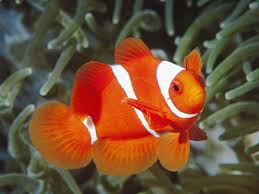
\includegraphics[width=0.95\textwidth]{nemo.jpeg} %% PARA COLOCAR O ARQUIVO DA IMAGEM NO SHARELATEX, CLIQUE NO ÍCONE QUE PARECE UMA FLECHINHA PARA CIMA (ATUALIZAR), CLIQUE EM UPLOAD E PROCURE A IMAGEM EM SEU COMPUTADOR.
\end{figure}



\subsection{Contexto e Problema}

Nesta sessão o aluno especificará qual o contexto onde o trabalho se encontra. Por exemplo, se for um trabalho na área de sistemas distribuídos, um possível contexto específico é a sub-área de middlewares, logo deverá falar um pouco deste conceito. 
Deverá ser dissertado aqui também qual o problema resolvido neste trabalho, porém apenas apresentando-o.


\subsection{Objetivos Gerais e Específicos}

O objetivo geral deste trabalho é apontar uma nova abordagem pedagógica para o melhoramento do processo de ensino e aprendizado, dos estudantes brasileiros do ensino médio e fundamental maior, através de um software que estou desenvolvendo, o qual  estimulará a competitividade entre os estudante, fazendo com que, estes sintam-se motivados a melhorar, causando assim uma ruptura na abordagem pedagógica vigente e o surgimento de uma nova pedagogia baseada na meritocracia. 

\begin{itemize}
\item Implantar o software e  sua pedagogia na Escola de Ensino Fundamental Jerônimo Alves Bezerra. 
\item Avaliar e realizar testes do  nível de  aprendizado dos estudantes, pré-implantação e pós-implantação do sistema.
\item Apresentar  relatórios  bimestrais do rendimento de cada aluno, a fim de averiguar a eficiência do sistema. 

\item Comparar os resultados obtidos por alunos exposto a nova pedagogia com da atual.
\item Fazer relatórios da opinião de pedagogos, professores e aluno em relação ao sistema. 
\item Apresentar conclusão científica a respeito eficiência ou ineficiência da pedagogia meritocrática com base nos relatórios e no comparativo das avaliações pré-implantação e pós-implantação do sistema, nos alunos de escola com acesso ao aplicativo e alunos de escolas que não tiveram contato com o mesmo.            
\end{itemize}


% ---
% Capitulo de revisão de literatura
% ---
\section{Referencial Teórico}

Mediante a problemática de baixos índices de aprendizado e uma taxa de reprovação alta, a solução que se apresenta consiste na intensificação de pedagogias voltadas para a meritocracia, incentivando os alunos a dedicarem o máximo de esforço. Para tanto a recompensa para este esforço não deve ser só passar de série, mas um prêmio que diferencie os melhores dos medianos. A consequência disto é uma punição para o não esforço mais significativa do que a simples reprovação. 
% --- Seção dentro do capítulo
\subsection{Baixo Nível da Educação Brasileira}
% ---
De acordo com que afirma CONSTANTINO (301 p. Privatize Já, 2012), A obsessão pela igualdade, não de oportunidades, mas de resultados por parte do Ministério da Educação e Cultura – MEC, tem ofuscado a meritocracia no ensino escolar consequentemente afetando o nível da educação brasileira que apresenta resultados pífios, para se constatar tal afirmativa, basta citar que a Organização para a Cooperação e Desenvolvimento Econômico – OECD em seu último relatório sobre educação em 2015 disponibiliza um ranking do nível de educação de 72 países, onde dos tais o Brasil apareceu na 60$^{o}$ posição. 

Embora possa se argumentar que  o fator principal para o baixo nível da educação no Brasil é a falta de investimento, os números informados pela OECD atestam o contrário, que o Brasil já investe mais do que a média dos países avaliados. O governo brasileiro destina 5,1\% do seu Produto Interno Bruto – PIB para educação, a média da OECD está em 4,8\%, e abrange em sumária maioria países ricos. O Japão, por exemplo, investe 3,3\%, a Alemanha 4\%, a Coreia do Sul, 4,5\%, o Canadá 4,6\% e a China 4\%. Isto provar que o debate teve transcender a questão econômica, deixar de lado a falácia de sempre que: “o governo investe pouco em educação” e reconhecer que na verdade investe mal. O ponto de reflexão a respeito da educação no Brasil deve ser a respeito do modelo pedagógico adotado pelo MEC e imposto a todas as escolas públicas do país, revisando a forma como os estudantes estão sendo educados. De maneira nenhuma  colocar mais dinheiro em um sistema que obviamente fracassou é adequado.  

Possuir a oportunidade de usar números como referencial para levantamento de hipótese é singular, afinal os números geralmente são irrefutáveis. Por tanto para acrescentar consistência à este trabalho é mister avaliar o Índice de Desenvolvimento da Educação Básica - IDEB de alguns estados brasileiros e avaliando o desempenho de algumas vertentes pedagógicas que corroboram para os melhores e piores resultados. Sem duvidas os melhores resultados são apresentados por São Paulo - SP e Santa Catarina - SC; com seus respectivos 4,7 e 4,9 no 9$^{o}$ ano  do ensino fundamental ; 6,2 e 6,1 no 5$^{o}$ do ensino fundamental; 4,2 e 3,8 no 3$^{o}$ ano do ensino médio. Os piores índices ficam por conta de: Alagoas - AL e Sergipe - SE; com seus respectivos 3,2 e 3,1 no 9$^{o}$ ano  do ensino fundamental; 4,3 e 4,1 no 5$^{o}$ do ensino fundamental; 3,1 e 3,2 no 3$^{o}$ ano do ensino médio.

% --- Seção dentro do capítulo
\subsection{Repetência Escolar}
% ---
 De acordo com o Instituto de Pesquisa Econômica Aplicada - IPEA: “desde 1996, quando a atual Lei de Diretrizes e Bases estabeleceu as normas fundamentais da educação nacional, se fala no fim da repetência escolar”.  A principal argumentação para o fim da reprovação escolar é que a reprovação provocaria altos índices de evasão escolar, mas os números apresentados pelo INEP atestam que os números de alunos repetentes matriculados no ensino médio chegaram 13,1\% em 2011 este é o maior índice desde 1999, mas apesar desta suntuosa alta o país apresenta queda 9,6\% no índice de evasão escolar. O que este índice de reprovação revela é a fragilidade da educação e onde se deve empregar esforços para melhorar a qualidade do ensino, mas o governo prefere lidar com sintomas ao invés de atacar as causas. 
 
Como bem expôs CONSTANTINO (309 p. Privatize Já, 2012): “O Governo vai lidando com sintomas, sem jamais focar nas causas do problema. Os mais pobres estudam em escolas que não oferecem qualidades de ensino para competir pelas vagas nas universidades federais? Então vamos criar cotas para arrombar a porta dos fundos dessas instituições! A taxa de repetência é elevada? Vamos acabar com ela. E assim por diante. O brasileiro parece acreditar que basta quebrar o termômetro para acabar com a febre do doente”. 

Quando o assunto é educação não existem soluções simplistas e para validar tal afirmativa basta analisar os Estados com menores índices de reprovação em 2011 foram Mato Grosso (3,6\%), Santa Catarina (4,4\%), São Paulo (4,9\%), Minas Gerais (7,3\%) e Goiás (7,6\%). Estados que apostaram em medidas de recompensa ao esforço e sucesso dos seus estudantes e professores.  Não precisaram eliminar a reprovação estudantil através de uma medida imediatista e arbitrária.


% --- Seção dentro do capítulo
\subsection{Meritocracia Na Educação}
% ---
Os estados que apresentam os melhores índices educacionais foram justamente os que realizaram projetos com algum grau de comprometimento com a meritocracia.   Mas em que consiste esta abordagem pedagógica, para entender é necessário exemplificar a etimologia das palavras  mérito e meritocracia. Pois o estudo léxico e sintático desses temos propiciará maior clareza do que se propõe este trabalho.  

Segundo Afirma (VIEIRA,2013) a palavra Mérito tem origem no latim meritum e designa tanto ganho, lucro quanto pena, castigo. “Ter mérito” é “quem é merecedor, ter mérito supõe ser digno de recompensa, elogio, prêmio, estima, apreço” (WALZER,2003).  Então supõe-se que só seriam louvados aqueles com amplitude de grandeza, ou seja, o ser que apresenta uma associação de qualidades intelectuais e morais reconhecidas pela sociedade, além de demonstrar grandioso esforço para ser merecedor de tais qualidades.  

A meritocracia em quanto doutrina foi descrita por (BARBOSA,2003) “como um conjunto de valores que postula que as posições dos indivíduos na sociedade devem ser consequência do mérito de cada um. Ou seja do reconhecimento público da qualidades das realizações individuais”.  A sentença meritocracia alude uma das mais conceituadas doutrina de fundamento de hierarquização, engloba inúmeros conglomerados da esfera pública. Sua aplicação científica na educação segundo (VIEIRA,2013) é “a única maneira de produzir desigualdades justas: se os indivíduos são fundamentalmente iguais, somente o mérito pode justificar as diferenças de remuneração, de prestígio, de poder, que influenciam as diferenças de desempenho escolar e do desempenho do professorado”. A meritocracia escolar desempenha uma Incumbência justificadora de hierarquias sócio-econômicas. (Bourdieu e Passeron,1975). 

A Meritocracia escolar é baseada nas filosofias iluministas, que conservam uma crença descomunal na educação, além da confiança no mérito como corporatura  principal da justiça escolar destinando-se a evidenciar os competentes e justificar suas posições (VIEIRA,2013).  Desta forma as pedagogias meritocráticas se resume em punição e galardão, por meio dessas condições os alunos são motivados a sempre melhorar. Para o professor torna-se mais fácil enxergar a quem deve dedicar mais do seu tempo e estímulos, justamente os que apresentam  piores resultados nas avaliações. 

A aprovação e reprovação é o centro da proposta deste projeto, incentivar os estudantes através de recompensas, gerando no âmbito escolar uma desigualdade justa. Onde aqueles que obtêm prêmios e vantagens por meio de seus esforços. Este mecanismo induz naqueles que não obtém êxito estimulados resultando em mais comprometimento  e aqueles que tiveram sucesso a continuar se esforçando. A quebra deste dispositivo resultaria em uma completa desestimulação dos estudantes  e consequentemente uma queda no rendimento. 



\section{Trabalhos Relacionados}

Lista trabalhos anteriores cujos temas sejam relacionados ao seu (forneça detalhes desses trabalhos apenas se tais detalhes ajudam a mostrar onde o seu trabalho é melhor do que eles; tenha certeza de mencionar todos os trabalhos relacionados, principalmente aqueles do pessoal do comitê de programa). Desvantagens ou pontos fracos de trabalhos anteriores que são aprimorados no trabalho sendo proposto. Condições e limitações do seu trabalho.


\section{Proposta}

Nesta parte do trabalho o aluno deve apresentar sua ideia principal.
A sessão de proposta marca o início da contribuição pessoal do autor do trabalho. Portanto, não se deve fazer desta sessão uma nova revisão bibliográfica. De preferência, todos os conceitos que serão necessários nesse capítulo já devem ter sido citados no capítulo de revisão bibliográfica. Se alguma comparação for feita com trabalhos correlatos nesse capítulo, então apenas a comparação objetiva deve ser feita
aqui, sendo que a apresentação pura e simples dos trabalhos correlatos já terá ocorrido na sessão anterior.
Esta sessão deve apresentar a construção da teoria, modelo ou proposta, seja de que
natureza for. Conceitos criados pelo autor do Trabalho de Conclusão de Curso devem ser descritos aqui e não na revisão
bibliográfica. Na sequência, o autor deve trabalhar as evidências de que sua hipótese é verdadeira. Serão então
apresentados dados, gráficos, testes, provas formais, estudos de casos, transcrição de entrevistas ou quaisquer
outros meios julgados adequados para provar o seu ponto, ou seja, para mostrar que a hipótese é verdadeira.
Deve-se evitar sempre transformar a sessão da proposta em uma apresentação de um sistema
computacional. Se um sistema foi desenvolvido, foi para servir a algum propósito de descobrir novo
conhecimento. A monografia deve ser sobre o conhecimento gerado, não sobre o sistema em si. Apresentações
detalhadas sobre telas de software, incluindo telas de login, menu principal etc., são enfadonhas e
desnecessárias em um trabalho científico. O seguinte texto, do Prof. J ohn W.Chinneck (1988), resume tudo:
“The purpose of your thesis is to clearly document an original contribution to knowledge. You may develop computer
programs, prototypes, or other tools as a means of proving your points, but remember, the thesis is not about the tool, it is
about the contribution to knowledge. Tools such as computer programs are fine and useful products, but you can’t get an
advanced degree just for the tool. You must use the tool to demonstrate that you have made an original contribution to
knowledge; e.g., through its use, or ideas it embodies.”

\subsection{Avaliação/Estudos de Caso}

Nesta parte do trabalho o aluno deverá apresentar como pretende avaliar o trabalho afim de comprovar suas hipóteses através de uma análise prática. 
Esta atividade poderá ser feita seguindo métodos de experimentos controlados ou mais simplesmente estudos de caso.


\section{Cronograma}

Descreva aqui as atividades que irá executar a cada mês.

\begin{table}[hbt] %% EXEMPLO DE TABELA FEITA POR MEIO DO http://www.tablesgenerator.com/
	\begin{center}
		\caption{Exemplo de Tabela.} %% LEGENDA (REPARE QUE ELE JÁ COLOCA A NUMERAÇÃO AUTOMATICAMENTE E JÁ ADICIONA À LISTA DE TABELAS
		\begin{tabular}{|l|l|lll}
			\cline{1-2}
			Atividade & Outubro   &  &  &  \\ \cline{1-2}\cline{1-2}
			 01 &   &  &  &  \\ \cline{1-2}
			 02  & X &  &  &  \\ \cline{1-2}
			 03    &  &  &  &  \\ \cline{1-2}
		\end{tabular}
	\end{center}
\end{table}

% ----------------------------------------------------------
% Referências bibliográficas
% ----------------------------------------------------------
\bibliography{abntex2-modelo-references}

\end{document}
